\section{Multimodal ArXiv}
This section presents a detailed construction process of our Multimodal ArXiv dataset, consisting of two sets: ArXivCap~(\S\ref{subsec:ArXivcap}) and ArXivQA~(\S\ref{subsec:arxiv_qa}).
% and then key statistics of the curated dataset.

% Figure~\ref{fig:chunk_example} illustrates a case sampled from our dataset.
% Step by Step?

% Use figure* for multi-column figure
\begin{figure*}[tp]
    \centering
    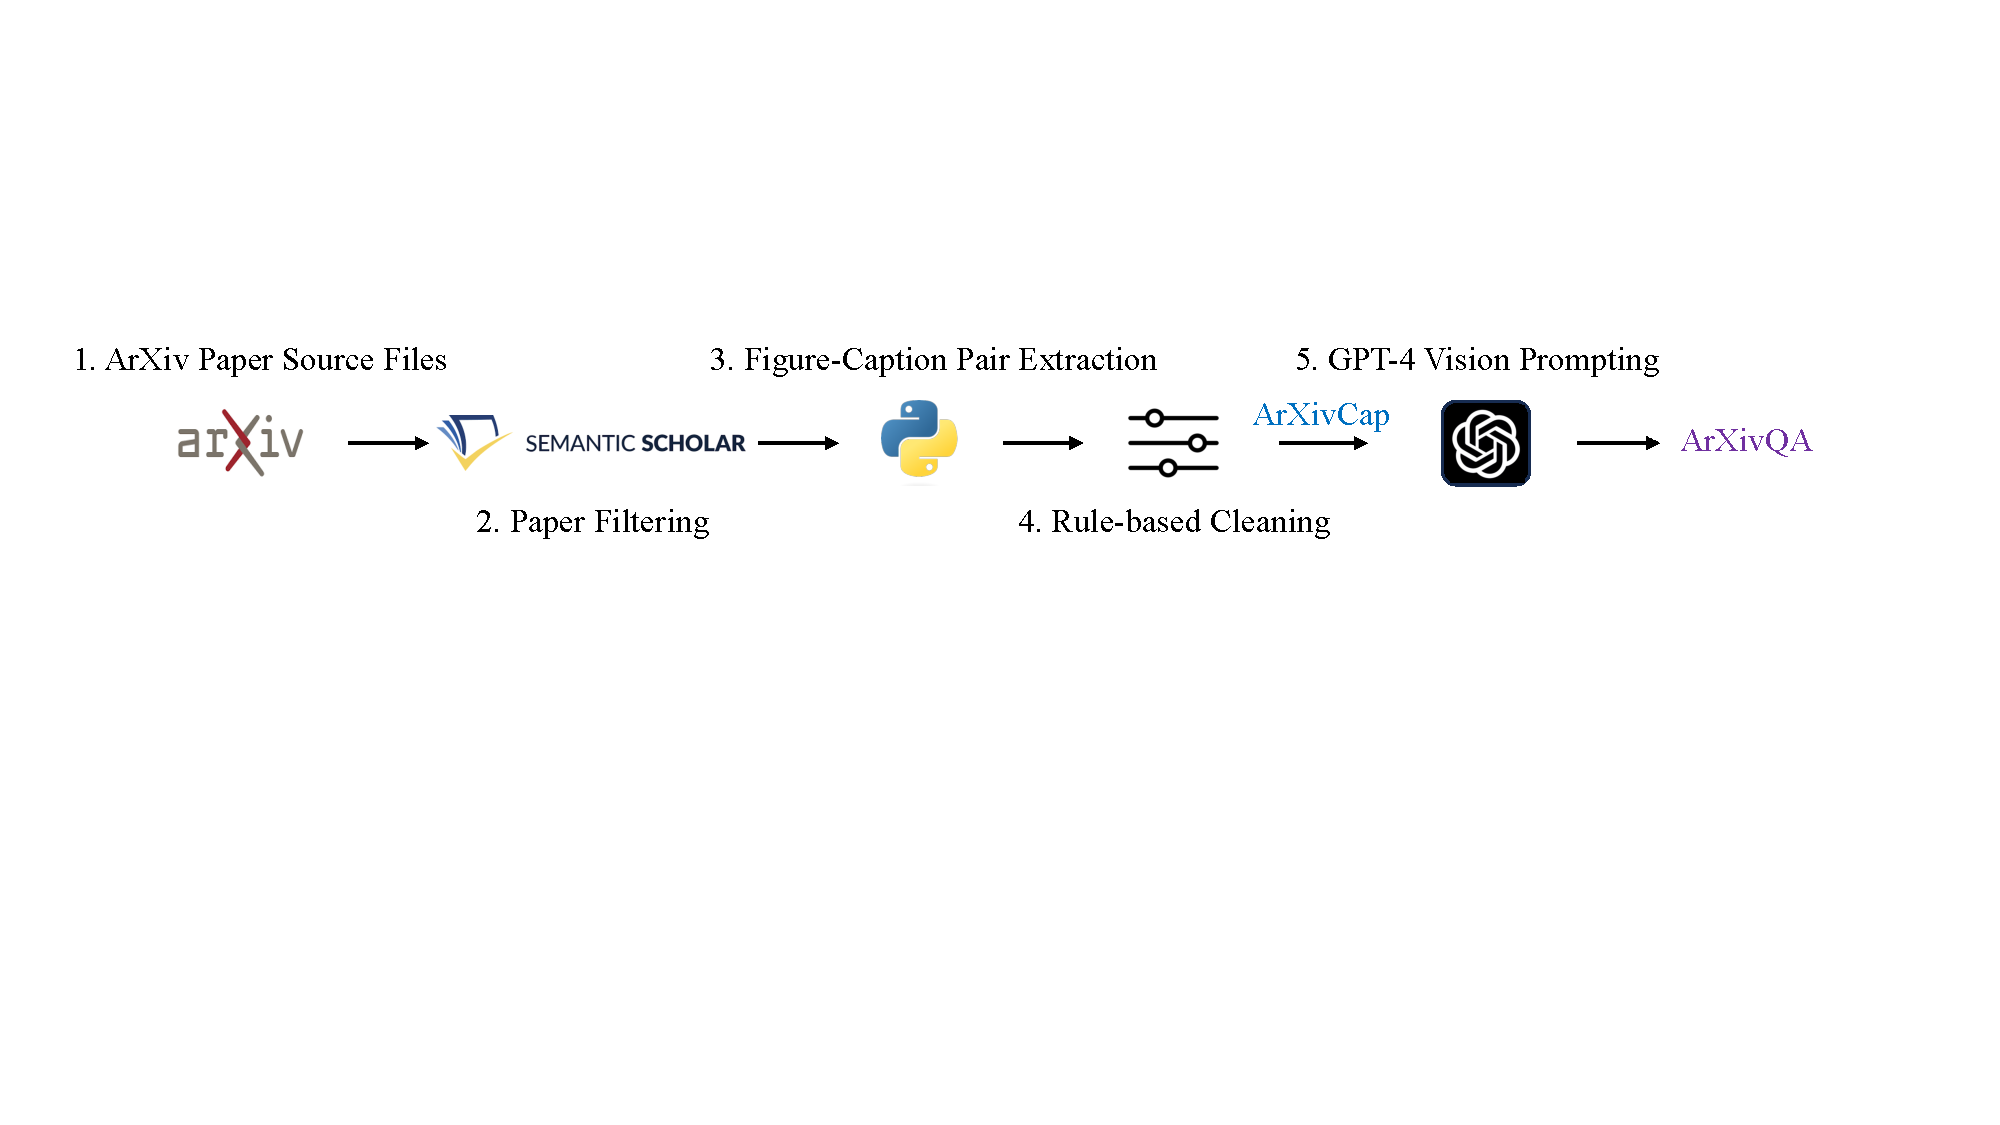
\includegraphics[width=0.95\linewidth]{figs/process.pdf}
    \caption{Overview of our dataset curation process. Starting from the ArXiv paper source files, we ensure the paper quality by selecting papers according to publication records. Figure and caption pairs are extracted and then cleaned according to manually designed rules. ArXivQA is generated by prompting GPT-4V with a curated template.}
    \label{fig:dataset-curation-process}
\end{figure*}


\subsection{ArXivCap}
\label{subsec:ArXivcap}

% \subsubsection{Construction Process of ArXivCap}
\paragraph{Construction Process} We outline the creation process of ArXivCap below and Figure~\ref{fig:dataset-curation-process} gives an overview.

\noindent\emph{Paper Filtering with Publication Type:}
\DatasetName is extracted from ArXiv~\cite{clement2019use}, which is under CC-0 licence for modification and distribution. 
% Therefore, we have the permission to create and distribute \DatasetName. 
% The files in the ArXiv dataset are in tar format, which includes LaTeX files and their corresponding image files. 
The raw files of papers posted on ArXiv tar files before June 2023 are downloaded. 
To ensure the quality of our dataset, we employ a rigorous selection process to filter potentially low-quality papers that might influence the figure-caption pair quality. 
Firstly, we retrieve meta-information for papers from Semantic Scholar~\cite{kinney2023semantic}, which contains the publication record for each paper. 
Papers with publication types \texttt{JournalArticle},  \texttt{Conference}, or \texttt{Review} are kept as we assume the peer-review process could ensure the overall figure-caption quality is satisfactory.
We further exclude papers with titles exceeding 100 words or abstracts longer than 300 words, in alignment with common submission requirements.
% We further filter out papers with titles longer than 100 words, or with an abstract longer than 300 words, according to common submission requirements.
% for examples. 
% There are 2,285,111 papers and 13,945,502 images in total till this step.


% % Use figure* for multi-column figure
\begin{figure}[!t]
    \centering
  \begin{subfigure}{0.45\textwidth}
    \centering
    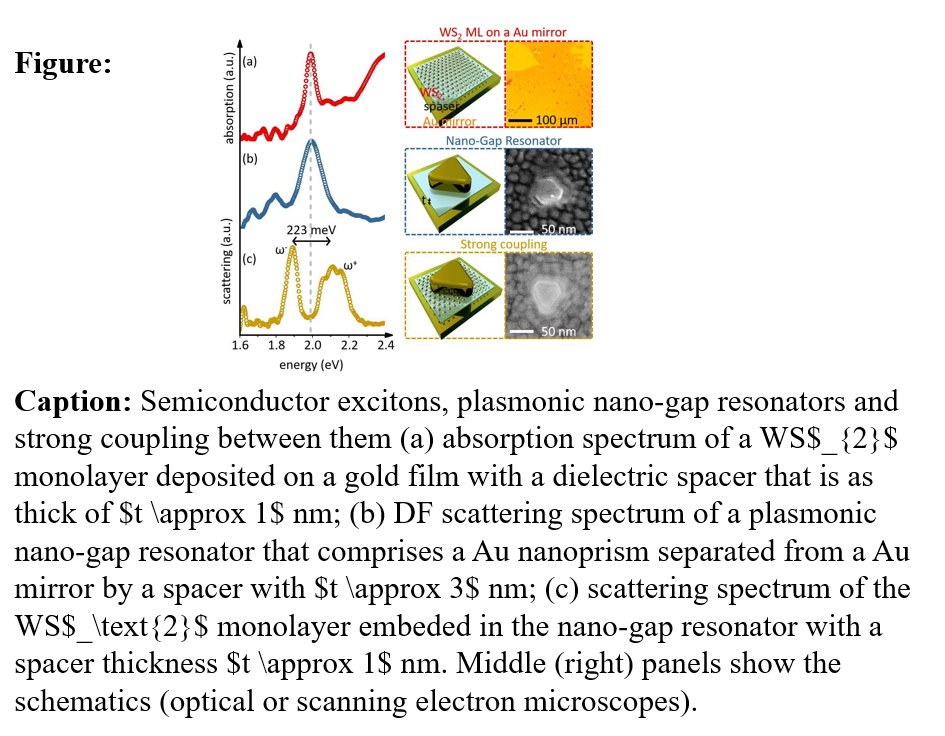
\includegraphics[width=\textwidth]{figs/examples/1-1.png}
    \caption{Single Figure-Caption}
    \label{fig:subfig1}
  \end{subfigure}
  \hfill
  \begin{subfigure}{0.45\textwidth}
    \centering
    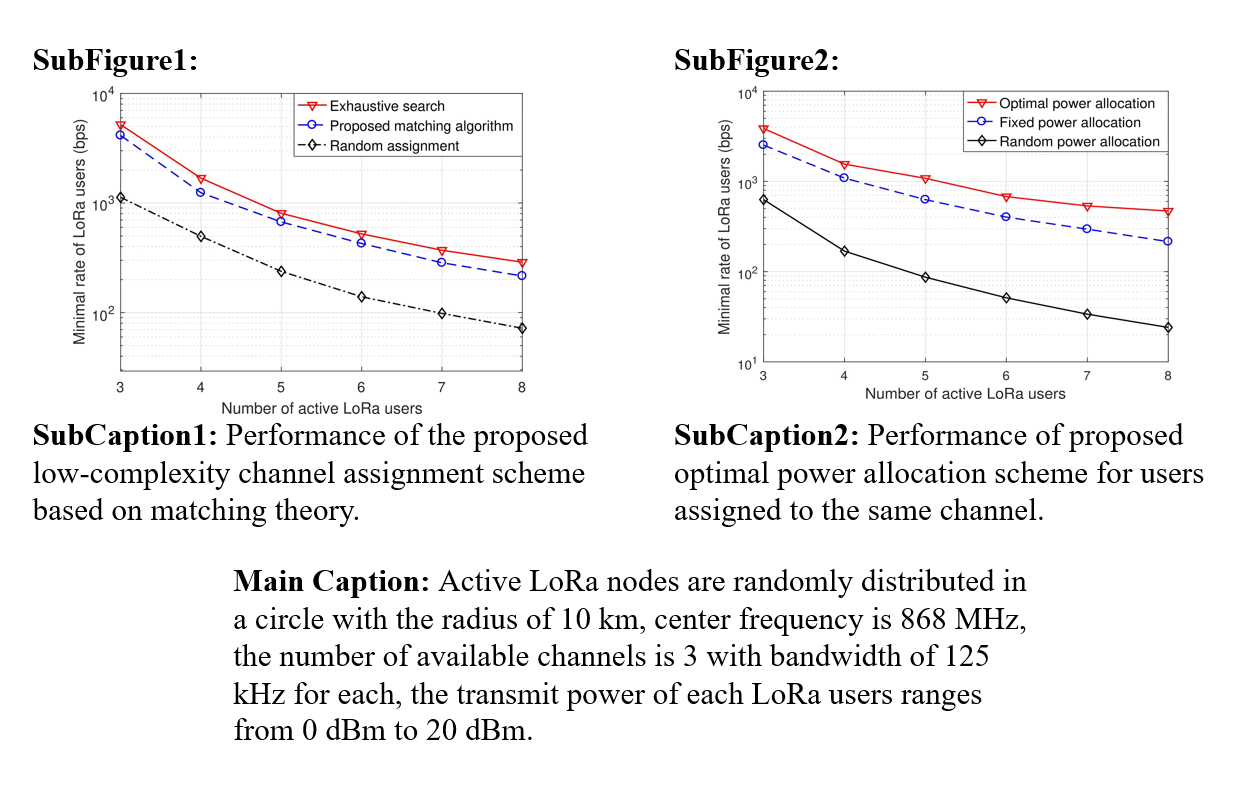
\includegraphics[width=\textwidth]{figs/examples/1-2.png}
    \caption{Multiple Figure-Caption}
    \label{fig:subfig2}
  \end{subfigure}
  \caption{Chunk Example. \lilei{add case of arxiv qa}}
  \label{fig:chunk_example}
\end{figure}

% \paragraph{Unify Image Format} 
% We utilize ImageMagisk~\cite{imagemagick} to convert images of various formats, including .ps, .epsi, .PS, .pdf, .PDF, .EPS, .eps, etc., into the JPEG format, while preserving the original jpg/jpeg and png images. ImageMagisk is a robust tool for image editing and transformation. Additionally, we standardize the output format to jpg/jpeg in RGB mode and remove the white border around images.

% according to our prior.
% This ensures that we include papers published in reputable journals, conference proceedings, or recognized review articles.
% We further keep papers satisfying the following requirements:
\noindent\emph{Figure-Caption Pair Extraction:}
Images and captions are extracted from the original LaTeX files by matching the syntax. 
We further use a robust tool ImageMagisk~\cite{imagemagick} to convert images into JPEG format for easy processing.
The extracted images and captions are stored in a designed chunk structure,
which consists of either a single figure-caption pair or multiple figures with their respective sub-captions and a main caption for the overall description.
This format is more consistent with the layout of academic papers, and
Figure~\ref{fig:chunk_example} illustrates the chunk structure.

% \begin{enumerate}% [leftmargin=2em]
%     \item The number of words in the abstract is in  $[10, 300]$.
%     \item The number of words in the title is in $[1, 100]$.
% \end{enumerate}

\begin{figure}[t!]
    \centering
    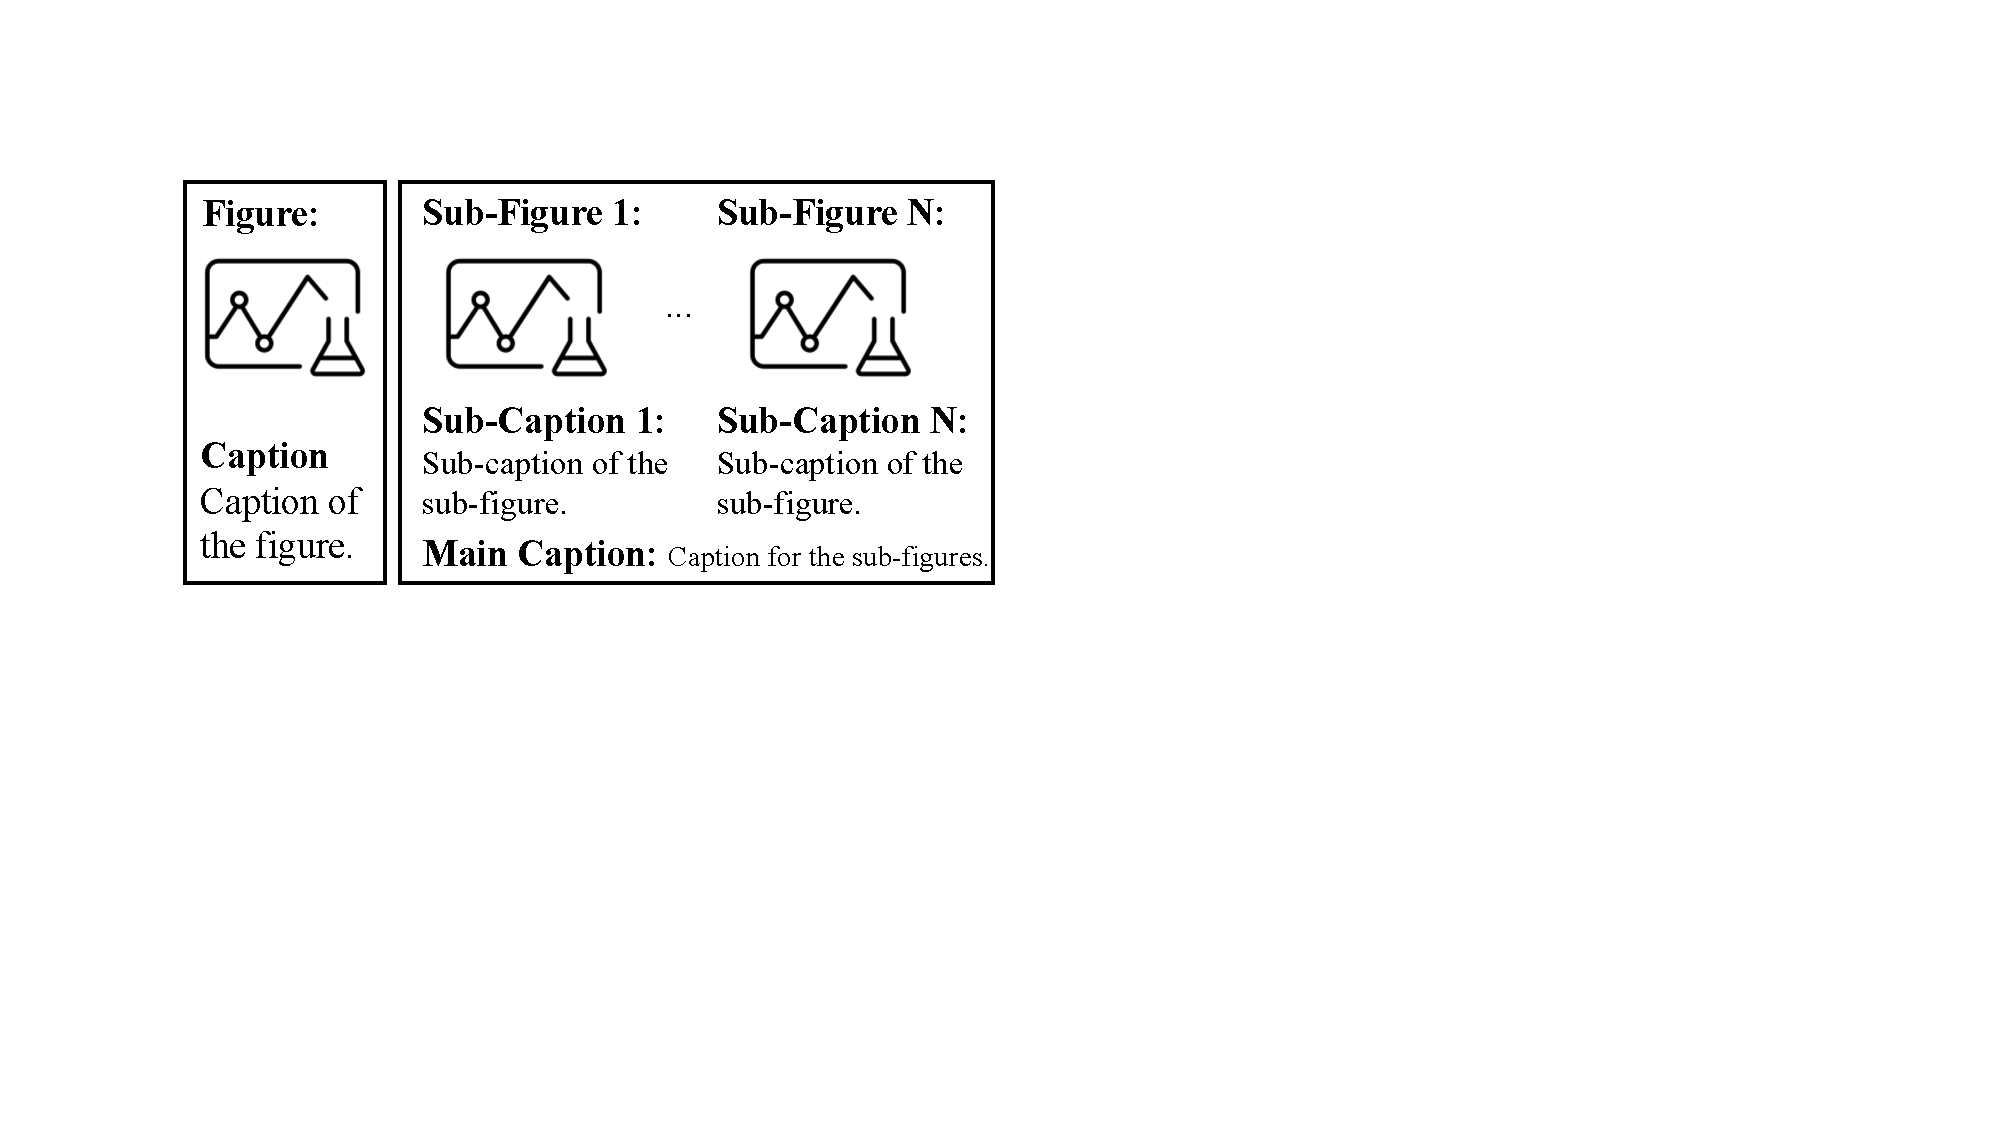
\includegraphics[width=0.9\linewidth]{figs/chunk-v2.pdf}
    \caption{Illustration of two types of figure-caption pairs. (Left) Single-Figure pair. (Right) Multiple-Figure caption pair has multiple sub-figures with corresponding sub-captions and an overall main caption. }
    \label{fig:chunk_example}
\end{figure}
% \paragraph{Filter Images}
% After resizing images using Lanczos resampling, we ensure that the maximum dimension of each image does not exceed 2016 pixels. Following a manual inspection of the images, we apply the following filters to refine the selection process further, retaining only the images that meet the specified requirements:

% \begin{enumerate}
%     \item The ratio between the width and height of the image is less than 100.
%     \item The width or height of the image is larger than 224 pixels.
%     \item The number of pixels in the image is less than 89,478,485.
% \end{enumerate}


\noindent\emph{Caption Cleaning and Image Filtering:}
After a manual inspection of the initially collected dataset, we design several transformations to clean the captions and filter the images.

\noindent\emph{Caption Cleaning}: (i) Chunks with captions shorter than 5 words are removed; (ii) For captions with LaTeX expressions such as math formulas and references, we apply the \texttt{pylatexenc}\footnote{https://github.com/phfaist/pylatexenc} to transform the LaTeX to text with math formulas retained, citations to a special symbol \texttt{<cit.>}, references to \texttt{<ref>}. An illustration of caption cleaning can be found in Appendix~\ref{apx:caption_clean}.
%\textgreater"


\noindent\emph{Image Filtering}: We remove images that are deemed to be problematic according to the following rules:
(i) Images with an aspect ratio larger than 100; (ii) Images with the shortest edge shorter than 224 pixels; and (iii) Images with pixel numbers larger than the decompression bombs threshold.
% The ratio between the width and height of the image is less than 100.
%     \item The width or height of the image is larger than 224 pixels.
%     \item The number of pixels in the image is less than 89,478,485.
% Replace incorrect newline characters with empty spaces.
    % \item Replace consecutive empty spaces with a single space.
    % Remove chunks that have captions with fewer than 5 words or no words at all.
   % Utilize pylatexenc to convert LaTeX to text, ensuring that math formulas are retained. Additionally, normalize citations and tables to "\textless ref \textgreater" and "\textless cit. \textgreater" format. (\cref{tab:pylatexenc_clean})
% \end{enumerate}

After these processes, 100 pairs are sampled to perform an additional manual inspection, where we found all of these pairs contained clear images and correct caption descriptions. We provide visualized figure-caption pairs in Appendix~\ref{apx:case_illustrations}.
\paragraph{Statistics of ArXivCap}
% In this section, we present a general analysis of \DatasetName. Detailed analysis can be found in the Appendix. 

% \begin{table*}[ht!]
    
%     \centering
    
%     \small 
%     \begin{tabular}{@{}lcccccc@{}}
%          \toprule
%         Field & Number & Total & Average & Minimum & Maximum & Quartile \\
%          \midrule
         
%         Title & 572,734 & 5,960,728 & 10.41 & 1 & 100 & (8, 10, 12) \\
                 
%         Abstract & 572,734 & 95,987,566 & 167.6 & 10 & 300 & (126, 165, 207) \\
        
%         Chunk Caption & 3,963,576 & 193,482,743 & 48.82 & 1 & 2,248 & (16, 36, 67) \\
        
%         Main Caption & 3,958,840 & 188,590,156 & 47.64 & 1 & 2,248 & (15, 35, 65) \\

%         Subcaption & 1,025,704 & 4,892,587 & 4.77 & 1 & 307 & (2, 3, 5) \\  

%         Images & 6,481,222 & N / A & N / A & N / A & N / A & N / A \\
%          \bottomrule
%     \end{tabular}
%     \caption{Word count statistics for title, abstract, captions and Image number. A word is defined as any sequence of characters matching the regular expression pattern r"\textbackslash w+". \cref{fig:chunk_example} shows the example of subcaption and main caption. The term "Chunk caption" encompasses all captions within it, including both the subcaption and the main caption contained within it.}
%     \label{tab:detail_statistic_title_abstract_image_caption}
% \end{table*}

\begin{table}[t!]
    \centering
    \resizebox{\linewidth}{!}{
    \begin{tabular}{@{}lccc@{}}
         \toprule
        Field & Number &  Average Len.  & Quartile of Len. \\
         \midrule
         
        Title & 572K &  10.4   & (8, 10, 12) \\ 
        Abstract & 572K &  167.6  & (126, 165, 207) \\
        \midrule 
        Main Caption & 3.9M  &  47.6 & (15, 35, 65) \\
        Subcaption & 1.0M  & 4.8 &  (2, 3, 5) \\  
        Chunk Caption & 3.9M &  48.8  & (16, 36, 67) \\
        \midrule 
        Images & 6.4M  & N / A  & N / A \\
         \bottomrule
    \end{tabular}}
    \caption{Word count statistics for title, abstract, captions, and Image number. 
    Chunk caption refers to the combination of subcaptions and the main caption for a multiple-figure case.}
    \label{tab:detail_statistic_title_abstract_image_caption}
\end{table}

\begin{table*}[ht!]
    \centering
\resizebox{\textwidth}{!}{
    \begin{tabular}{@{}lccccc@{}}
         \toprule
        Dataset & Image Number & Paper Number & Image Category & Domain & Real Data \\
         \midrule
                 FigCAP~\citep{chen2020figcap} & 219K & N / A & Bar, Line and Pie Charts & N / A & \xmark \\
        
         SciCap~\citep{Yang2023SciCap+} & 2.1M & 295K & Open-Category & Computer Science and Machine Learning & \cmark \\

         M-Paper~\citep{hu2023mplugpaperowl} & 350K & 48K & Open-Category & Mainly "Deep Learning" & \cmark \\   
        
         ArXivCap (Ours) & 6.4M & 572K & Open-Category & Open-Domain & \cmark \\
 
        \midrule 
FigureQA~\citep{kahou2017figureqa}  & 140K & N / A & Bar, Line and Pie Charts & N / A & \xmark \\
                 
        DVQA~\citep{kafle2018dvqa} & 300K & N / A & Bar Charts & N / A& \xmark \\
         ArXivQA (Ours) &  32K & 16.6K & Open-Category & Open-Domain & \cmark \\
         \bottomrule
    \end{tabular}}
    \caption{Comparison with previous scientific figure datasets. Our ArXivCap is the largest captioning dataset and our ArXivQA is the only QA dataset that covers a wide range of domains from real papers. }
    \label{tab:dataset_comparison_1}
\end{table*}

% \crossmark & \cmark 

Table~\ref{tab:detail_statistic_title_abstract_image_caption} lists the dataset statistics. 
ArXivCap consists of 572K papers, containing 6.4M high-quality images in total with 193M words. 
A word cloud illustration of captions can be found in the Appendix~\ref{apx:caption_word_cloud}.
Figure~\ref{fig:domain-distribution} demonstrates the paper domain distribution extracted from ArXiv, where we find that our ArXivCap covers 32 domains, such as computer science, mathematics, physics, and economics.
As shown in Table~\ref{tab:dataset_comparison_1}, compared with previous scientific figure datasets, our ArXivCap is the largest figure-caption dataset collected from real papers and covers a wide range of scientific domains, serving as a valuable resource for improving and benchmarking LVLMs.

%, and our ArXivQA is the only open-domain QA datasets with diverse figure types.

% , providing a comprehensive general knowledge for LVLMs.

% It is the largest image-caption dataset for academic figures, encompassing a diverse array of domains and image categories. \cref{tab:dataset_comparison_1} presents comparison between \DatasetName and other datasets.
 % We get the domain category for each paper from \cite{ArXiv.org_submitters_2023}. 



% \begin{table}[tbh!]
    \centering
    \begin{tabular}{l|c}
    \toprule
       Field  & Total Number \\
       \midrule
       Title \& Abstract & 572,734 \\ 
       Image & 6,481,222 \\ 
       Caption & 3,961,133 \\ 
       \bottomrule
    \end{tabular}
    \caption{Data Statistics of the curated dataset.}
    \label{tab:data_statistics}
\end{table}

\begin{table}[tbh!]
    \centering
    \begin{tabular}{l|cc}
    \toprule
       Field  & Total Number & Word Number \\
       \midrule
       Block Caption & 3,963,576 & 193,482,743 \\ 
       Main Caption in Block & 3,958,840 & 188,590,156 \\ 
       Subcaption in Block & 1,025,704 & 4,892,587 \\ 
       \bottomrule
    \end{tabular}
    \caption{Caption Statistics of the curated dataset.}
    \label{tab:caption_statistics}
\end{table}


% \begin{table}[tbh!]
%     \centering
%     \begin{tabular}{l|cc}
%     \toprule
%        Field  & Statistic \\
%        \midrule
%        Image Number & 6,481,222 \\ 
%        Total Size & 892GB \\ 
%        \bottomrule
%     \end{tabular}
%     \caption{Image Statistics of the curated dataset.}
%     \label{tab:image_statistics}
% \end{table}


% Use figure* for multi-column figure
\begin{figure}[t!]
    \centering
    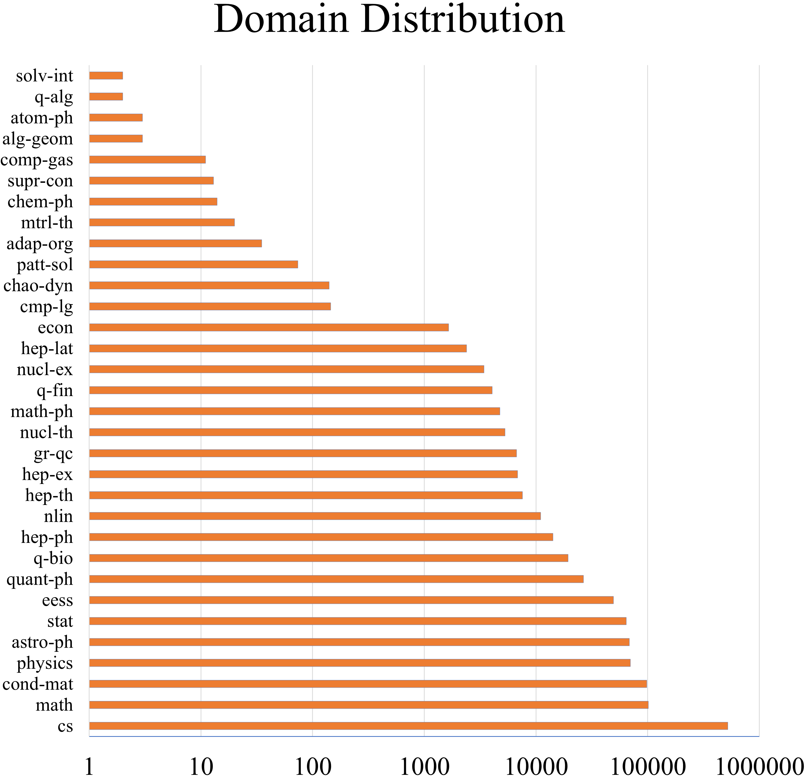
\includegraphics[width=0.9\linewidth]{figs/domain-distribution_500.png}
    \caption{Paper domain distribution of ArXivCap. See Table~\ref{tab:domain-full-name} in Appendix~\ref{apx:arxiv_cap} for the full name of each domain.}
    \label{fig:domain-distribution}
\end{figure}


\subsection{ArXivQA}
\label{subsec:arxiv_qa}
As our ArXivCap contains diverse images from scientific domains, we assume that learning to answer questions about these figures could boost scientific reasoning ability. Following the successful practice of LLaVA~\citep{liu2023llava}, we adopt GPT-4V to generate instruction-tuning datasets for generating the QA pairs based on the figures extracted from scientific papers.
Specifically, we design a prompting template to query GPT-4V for generating QA pairs based on 35K images randomly sampled from our ArXivCap.
Table~\ref{tab:prompt_for_ArXivqa} in Appendix~\ref{apx:prompt_template} provides the template we used for the prompt.
The generated pairs are parsed according to the format requirement and we discard the samples without options and rationales.
There are 100K QA pairs after filtering the invalid samples. 
The dataset comprises questions with an average word count of 16.98 for the question text.
% and options for the question with an average word count of 31.86. 
On average, there are 4.20 options per question and the average length of the text for a single option is 7.59 words.
Appendix~\ref{apx:case_illustrations} provides samples from the ArXivQA dataset.

As a preliminary study, we sample 1,000 samples from ArXivQA and prompt open-sourced LVLMs to predict answers given the questions and options. 
A simple prompt is designed to employ GPT-4 for extracting the answer label from the model generations.
For human performance, we ask four authors to perform predictions on a 100-sample subset (where 17 samples are from the CS domain). Each of them is asked to answer 50 samples and the accuracy scores are obtained by averaging two annotators.
As shown in Table~\ref{tab:arxiv_qa_acc}, most models struggle to perform satisfactorily on the ArXivQA dataset, falling far behind human performance. This verifies our premise that current open-sourced LVLMs fail to understand scientific figures. We also notice that simply increasing the model scale from 7B (LLaVa-1.5-7B) to 13B (LLaVa-1.5-13B) does not yield a significant boost, which indicates that the ability for multimodal mathematical reasoning cannot be simply acquired from the LLM-side only. 




\begin{table}[t!]
    \centering
    \small 
    \begin{tabular}{l|c}
        \toprule
        Model & Accuracy \\
        \midrule
        InstructBLIP-Vicuna7B & 7.0\% \\
        LLaVA-1.5-7B & 44.2\% \\
        LLaVA-1.5-13B & 46.8\% \\
        OpenFlamingo-9B & 9.9\% \\
        IDEFICS-Instruct-9B & 34.5\% \\
        Qwen-VL-Chat & 46.6\% \\
        \midrule 
        \textcolor{gray}{Human (100-sample Subset)} & \textcolor{gray}{80.0\%} \\
        \textcolor{gray}{Human (CS subset)} & \textcolor{gray}{88.2\%} \\
        \bottomrule
    \end{tabular}
    \caption{Evaluation results on the sampled 1,000 ArXivQA samples. }
    \label{tab:arxiv_qa_acc}
\end{table}
% Domain and Option Number, Option length, verb visualization?


